\documentclass[tikz,border=8pt]{standalone}
\usepackage[utf8]{inputenc}
\usetikzlibrary{positioning,fit,arrows.meta,shapes.geometric}
\definecolor{navy}{HTML}{17365D}\definecolor{teal}{HTML}{1F7A8C}\definecolor{soft}{HTML}{EAF4F6}
\tikzset{actor/.style={draw=navy,rounded corners,fill=white,minimum width=3.3cm,minimum height=.75cm,font=\bfseries\small},
usecase/.style={draw=teal,ellipse,fill=soft,minimum width=5.8cm,minimum height=.72cm,align=center,font=\small},
link/.style={draw=navy,-{Latex[length=2mm]},thin}}
\begin{document}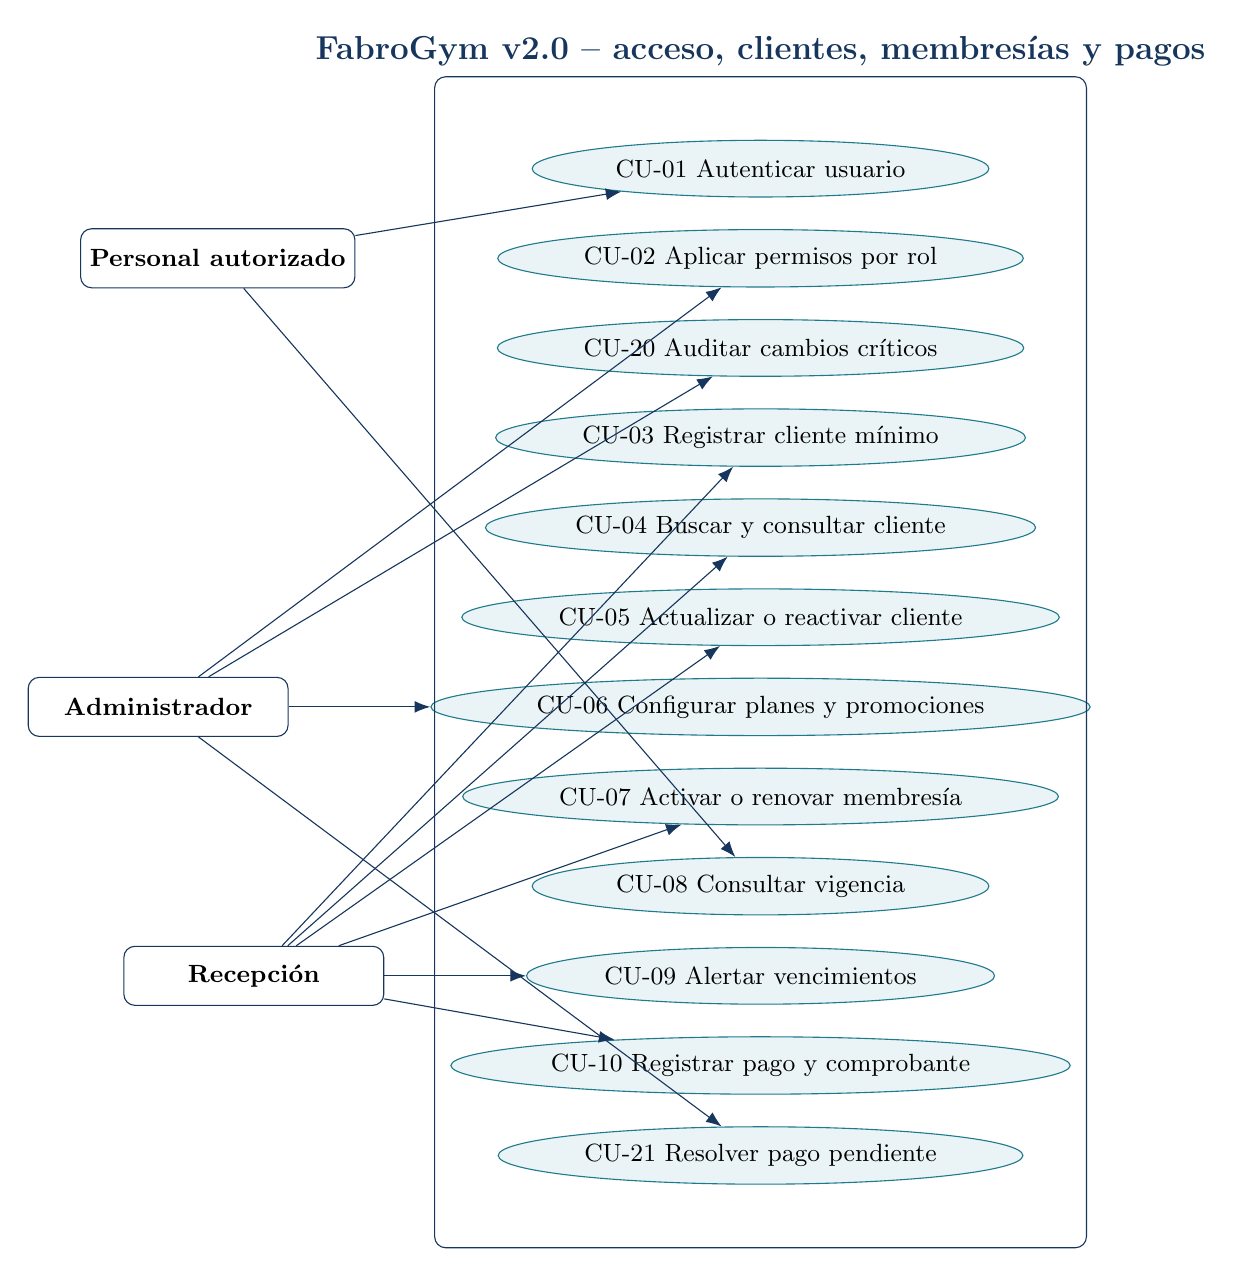
\begin{tikzpicture}[node distance=4mm and 14mm]
\node[usecase] (c1) {CU-01 Autenticar usuario};
\node[usecase,below=of c1] (c2) {CU-02 Aplicar permisos por rol};
\node[usecase,below=of c2] (c20) {CU-20 Auditar cambios críticos};
\node[usecase,below=of c20] (c3) {CU-03 Registrar cliente mínimo};
\node[usecase,below=of c3] (c4) {CU-04 Buscar y consultar cliente};
\node[usecase,below=of c4] (c5) {CU-05 Actualizar o reactivar cliente};
\node[usecase,below=of c5] (c6) {CU-06 Configurar planes y promociones};
\node[usecase,below=of c6] (c7) {CU-07 Activar o renovar membresía};
\node[usecase,below=of c7] (c8) {CU-08 Consultar vigencia};
\node[usecase,below=of c8] (c9) {CU-09 Alertar vencimientos};
\node[usecase,below=of c9] (c10) {CU-10 Registrar pago y comprobante};
\node[usecase,below=of c10] (c21) {CU-21 Resolver pago pendiente};
\node[draw=navy,rounded corners,fit=(c1)(c21),inner sep=8mm,label={[font=\bfseries\large,text=navy]above:FabroGym v2.0 -- acceso, clientes, membresías y pagos}] (sys) {};
\node[actor,left=18mm of c2] (pa) {Personal autorizado};
\node[actor,left=18mm of c6] (ad) {Administrador};
\node[actor,left=18mm of c9] (re) {Recepción};
\draw[link] (pa)--(c1); \draw[link] (pa)--(c8);
\foreach \x in {c2,c20,c6,c21}\draw[link] (ad)--(\x);
\foreach \x in {c3,c4,c5,c7,c9,c10}\draw[link] (re)--(\x);
\end{tikzpicture}\end{document}
